\section{Introduction} \label{sec:intro}
Monitoring and modeling of large-scale stochastic phenomena with both spatial and temporal (spatiotemporal) evolution using a network of distributed sensors is a fundamental problem in the applied sciences.   Consider for example a team of mechanical weeding robots managing herbicide resistant weeds on a farm (see Figure \ref{fig:cps}). This team of robots needs to predict the weed growth across the whole farm in real time to make intelligent decisions on robot coordination \cite{McAllistar18IROS}. With rapid advances in robotics and the capability to process large volumes of data on compact computational packages, the applications for such distributed Cyber Physical Systems are rapidly expanding. Common examples include modeling and monitoring ocean heat content and acidification in oceanography using a network of satellites and surface sensors; prediction of traffic patterns using data from vehicles, cellphones, and traffic cameras; prediction of enemy movements through ground and aerial surveillance, and prediction of spatiotemporal evolution of extreme weather events using data from weather stations and aerial drones. % \cite{barnett2001detection}future seismicity \cite{bungum2005postglacial}, land use change in urbanization \cite{deng2009spatio}, and extreme weather events \cite{heaton2011spatio}. One emerging and compelling example is 
 
\begin{figure}[h] %{r}{0.5\textwidth}
	\centering
	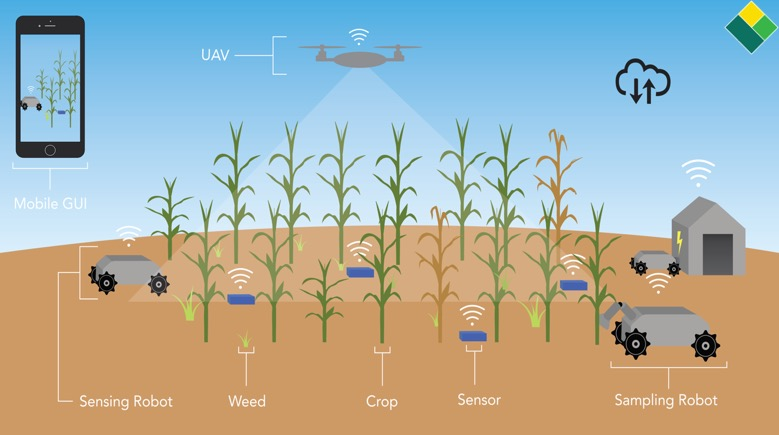
\includegraphics[width=\columnwidth]{agrobot_cps.jpg}
		\caption{A Cyber Physical system consisting of a distributed team of robots for mechanical weed management on a farm. Image courtesy EarthSense inc.}
	\label{fig:cps}
\end{figure}
%With rapid advances in low-cost data processing hardware and mobile robotics, large scale cyber physical systems capable of monitoring 

 %In situations where this is possible, such as in computational fluid dynamics, the resulting models may become computationally intractable, requiring hours or even days on supercomputers, and far out of the reach of compute and connectivity capabilities on robots or sensors deployed in the field.  On the other hand, recent advances in machine learning indicate that perhaps data-driven modeling could be a promising way  .  


%There has been significant interest in developing distributed modeling and monitoring algorithms for such systems, however, 


%The objective of this article is to introduce a modeling and monitoring mechanism that marries together recent successes of machine learning with powerful results from systems and control theory. We achieve this by demonstrating how critical properties such as observability and controllability can be derived systems can be embedded inside feature spaces of machine learning models We now elaborate the context behind this claim.  
% Let us dwell on this point a bit, its rather tempting to dismiss deep learning models and machine learning in general as blackboxes, but one can't argue with the success of those models. Taking a deeper look, one realizes that all machine learning is trying to do is to automatically learn a state-space (termed as the feature space cite our sidebar) which may be nonlinarly generated using other features. Infact sidebar blabla discusses three ways in which one could come up with these features, what the engineering community prefers is the features of the first kind which are physically directly relatable to physical quantities. 
%The success of machine learning in complex problems teaches us that giving up on interpretability allows one to solve very tough problems. SO its not the feature space that's the problem, 
%When one gives up physical interpretability, it becomes rather  difficult to understand why something is broken, or what guarantees could be put in place to ensure performance remains within bounds. with the traditional deep learning models, the only real way of dealing with this right now is sampling based, that is through thousands of simulations. Going a step further, its difficult to come up with guarantees on certain behaviors of the model. Observability and controllability are two fundamental guaratnees that controls interpretable models have provided us. SO the question that we ask here is does embedding interpretable models in complex feature spaces allows us to recover some of those guarantees while leveraging the strength of feature learning.

%Taking a broader perspective, complex dynamical systems such as agriculture and weather are very difficult to model and control using traditional first principles based approaches alone. On the other hand


These types of problems are characterized by complex and stochastic dynamics that are distributed in space and time. %It may be difficult to model such systems with spatiotemporal dynamics using first principles alone. 
While modeling such spatiotemporal phenomena has traditionally been the province of the field of geostatistics, it has in recent years gained more attention in the machine learning community \cite{cressie2011statistics}. The data-driven models developed through machine learning techniques provide a way to capture complex spatiotemporal phenomena which are not easily modeled by first-principles alone. 


 %, such as those described by stochastic partial differential equations with uncertain parameters. %, such as stochastic partial differential equations. 

In the machine learning community, kernel methods represent a class of extremely well-studied and powerful methods for inference in spatial domains; in these techniques, correlations between the input variables are encoded through a covariance kernels, and the model is formed through a linear weighted combination of the kernels \cite{RasmussenWilliams2005,schoelkopf01kernelbased,scholkopf2002learning}. In recent years, kernel methods have been applied to spatiotemporal modeling with varying degrees of success \cite{cressie2011statistics,RasmussenWilliams2005}. Many recent techniques in spatiotemporal modeling have focused on nonstationary covariance kernel design and associated hyperparameter learning algorithms \cite{garg2012AAAI,ma2003nonstationary,plagemann2008nonstationary}. These methods, which focus on the careful design of covariance kernels,  have been proposed as an alternative to the naive approach of  simply including time as an additional input variable in the kernel \cite{Chowdhary13_CDC1}. The careful design/optimization of covariance kernel avoids an explosion in the number of parameters (kernels utilized) of the model which would be inevitable in a model that simply adds time as an additional input variable, and has been shown to better account for spatiotemporal couplings. However, there are two key challenges with existing kernel based approaches: The first is ensuring the scalability of the model to large scale phenomena, which manifests due to the fact that the problem of optimizing the covariance kernel (known as hyperparameter optimization in the ML community) is not convex in general, leading to methods that are difficult to implement especially in online settings, susceptible to getting stuck at local minima, and highly computationally demanding for large datasets. % \cite{sra2012optimization}. 
The second key challenge is in using existing kernel-based machine learning models for analysis and synthesis of observers and controllers for the large scale spatiotemporal phenoemena. While the first challenge can be addressed with increasing computational power for large datasets, addressing the latter (and vastly more fundamental) challenge is particularly important in the design of reliable engineering systems, such as distributed sensor/actuator networks intended for monitoring physical phenomena, autonomous soft-robots, or other physical systems with distributed sensing and actuation.  %Consider in specific the problem of designing an optimal distributed sensor network for ``monitoring'' a spatiotemporally evolving function. 
%Some of the fundamental engineering questions that are of importance here are Given an approximate predictive model of the spatiotemporal phenomena, how can the current latent state of the phenomena be estimated using as few sensor measurements as possible?  
% 
   
%In addition to the challenge of modeling spatiotemporally varying processes, we are interested in addressing the second very important, and widely unaddressed challenge:

%To focus the development of the theory, we posit the challenging problem of ``monitoring'' a spatiotemporal phenoemena: Given an approximate predictive model of the spatiotemporal phenomena, how can the current latent state of the phenomena be estimated using as few sensor measurements as possible? This is called the \emph{monitoring problem}. Monitoring a spatiotemporal phenomenon is concerned with estimating its current state, predicting its future evolution, and inferring the initial conditions utilizing limited sensor measurements. The key challenges here manifest due to the fact that it is typically infeasible or expensive to deploy sensors at a large scale across vast spatial domains. %For example, in monitoring the flux of $CO_2$ over underground $CO_2$ storage sites, the number of sensors and sensing locations are limited due to cost or geography. %In another example, when monitoring the state of dynamically evolving enemy deployment over a contested area, the availability of measurements is limited due to the presence of adversity.
%To minimize the number of sensors deployed, a predictive data-driven model of the spatiotemporal evolution could be learned from historic datasets or through remote sensing  (e.g. satellite, radar) datasets. Then, to monitor the phenomenon, the key problem would boil down to reliably and quickly estimate the evolving latent state of the phenomena utilizing measurements from very few sampling locations.

%The problem of state estimation of a temporally evolving finite-dimensional state-space system has been extensively studied in the dynamical systems and feedback-control community \cite{Gelb74}. Fundamental results in systems observability theory provide sufficient conditions on the structure of the state transition and measurement matrix such that the latent state can be tracked with a measurement-feedback observer using a number of measurements less than the number of states. A highly successful example of such a state estimator is the celebrated Kalman filter, which is a Bayes-optimal filter for estimating the latent states of a finite-dimensional linear state-space model corrupted with Gaussian noise \cite{Gelb74}. Such filters can be extended to the functional domain \cite{mardia1998kriged}, but are typically not studied in a monitoring context. 


\subsection{Contributions}
In this article, we present a new perspective to solving the spatiotemporal monitoring problem that brings together kernel-based modeling, systems theory, and Bayesian filtering. We define the monitoring problem as follows: \textit{Given an approximate predictive model of the spatiotemporal phenomena learned using historic data, estimate the current latent state of the phenomena in the presence of uncertainty using as few sensors as possible}. In particular, we argue that when it comes to predictive inference over spatiotemporal phenomena, a Kalman-filter type approach of predicting and correcting with feedback from a set of minimal sensors is a robust way of dealing with real-world uncertainties and inherent modeling errors.  In the context of this specific problem, our \textit{main contributions are two-fold}: first, we demonstrate that spatiotemporal functional evolution can be modeled using stationary kernels with a linear dynamical systems layer on their mixing weights. In particular, in contrast with existing work, this approach does not necessarily require the design of complex spatiotemporal kernels, and can accommodate positive-definite kernels on any domain on which it is possible to define them, which includes non-Euclidean domains such as Riemannian manifolds, strings, graphs and images \cite{Jayasumana_PAMI2015_RBFs}. Second, we show that such a model can be utilized to determine sensing locations that guarantee that the hidden states of functional evolution can be estimated using a Bayesian state-estimator (Kalman filter) with very few measurements. We provide sufficient conditions on the number and location of sensor measurements required and prove non-conservative lower bounds on the minimum number of sampling locations by developing fundamental results on observability of kernel based models. The validity of the presented model and sensing techniques is corroborated using synthetic and large real datasets. (MENTION DNNS)

\subsubsection*{Broader Context}
The fundamental idea of building observers and controllers introduced in this paper is generalizable beyond the particular application of spatiotemporal monitoring. Indeed, the significance of the contributions of this paper are in fusing machine learning theory with systems theory to provide a pathway to address major challenges in distributed monitoring and control of complex spatiotemporally varying systems. 


\begin{figure}[h] %{r}{0.5\textwidth}
	\centering
	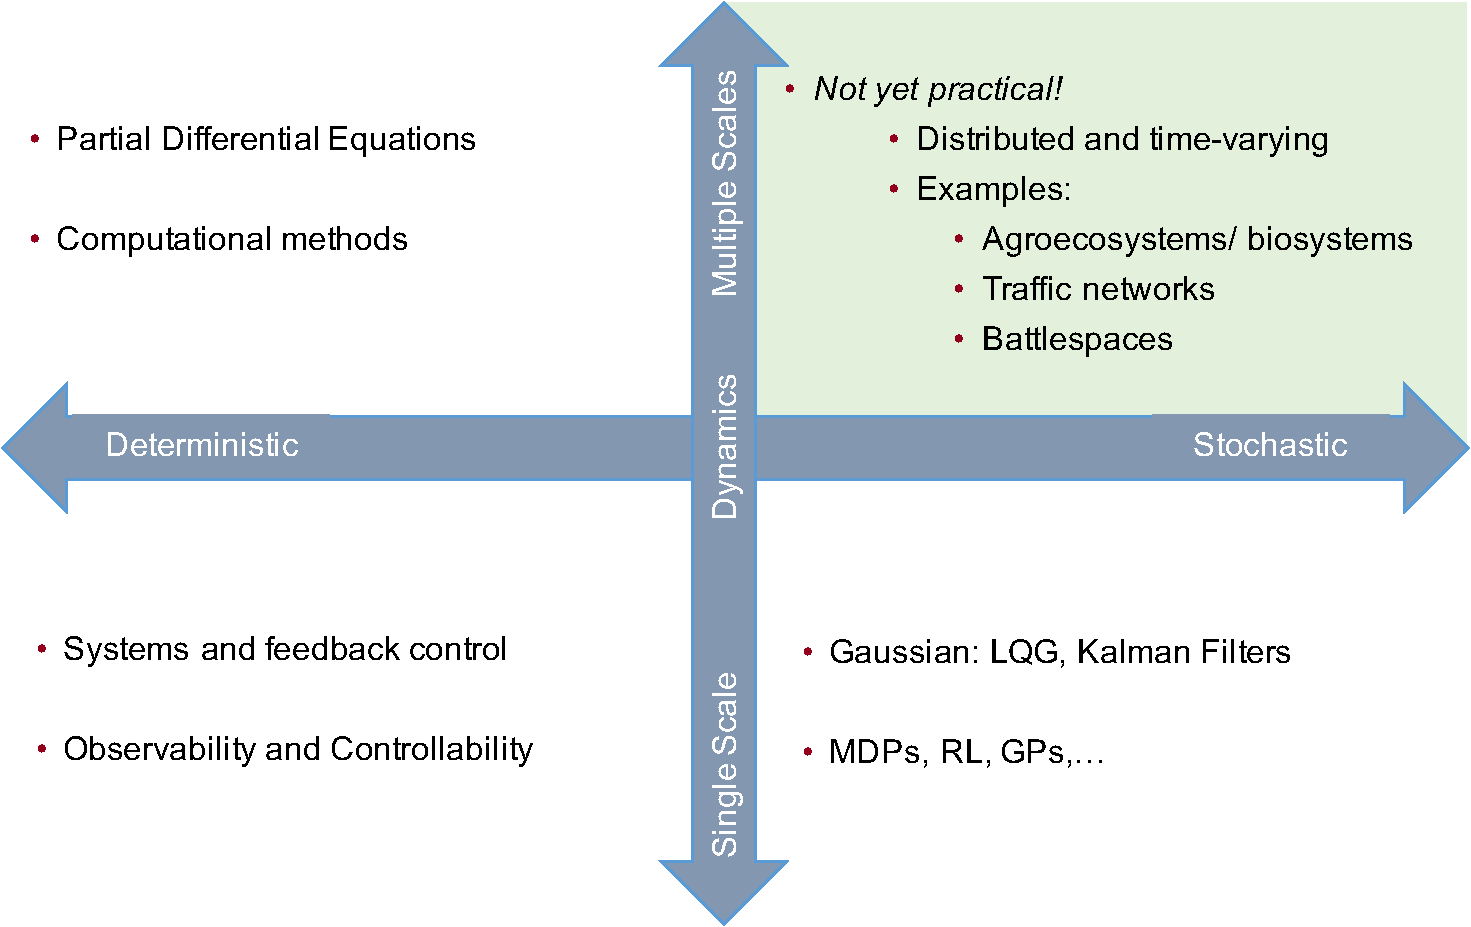
\includegraphics[width=\columnwidth]{CPS_SOA}
		\caption{Modeling, monitoring, and controlling dynamical systems with complex and uncertain dynamics, such as agricultural, traffic, or weather monitoring systems, presents exciting open challenge for the controls community. The bottom left quadrant describes linear and time-invariant systems with single- scale dynamics, for which the theory of feedback control of dynamical systems is often sufficient. The bottom right quadrant shows stochastic single-scaled systems, where approaches such as Kalman Filters and Gaussian optimization have marked several successes of control systems enabling endeavors from Lunar landings to GPS navigation. The top left quadrant denotes systems with dynamics at multiple scales, where efficient computational solutions to Partial Differential Equations (PDEs) is an highly active area of research. However, fundamental theoretical advances and practical algorithms are needed to enable autonomous decision making for distributed stochastic Cyber Physical Systems with dynamics at multiple scales – shown in the top right quadrant – such as distributed agricultural robotic systems, traffic networks, and weather monitoring systems with mobile and stationary sensors.}
	\label{fig:cps_soa}
\end{figure}
%Complex spatiotemporally varying systems such as agricultural systems, weather patterns, or fluid flows are typically difficult to address with traditional controls model with
  
Traditionally, the controls literature is strongest when the system dynamics can be represented as ODEs. % (see for example Figure \ref{fig:cps_soa}. Indeed %has focused on first principles and physics based models. As 
As depicted in Figure \ref{fig:cps_soa}, some of the major successes of controls have included results such as LQG, reinforcement learning, and adaptive control in finite, well-defined, and physically meaningful state spaces. The problem of state estimation of a temporally evolving, finite-dimensional state-space system for example has been extensively studied in the context of Kalman filtering and observer design \cite{Gelb74}. Here, fundamental results in observability/controllability provide sufficient conditions on the structure of the state transition and measurement matrix such that the latent state can be estimated in the presence of measurement and process noise. %A highly successful example of such a state estimator is the celebrated Kalman filter, which is a Bayes-optimal filter for estimating the latent states of a finite-dimensional linear state-space model corrupted with Gaussian noise \cite{Gelb74}. 
Such filters can be naively extended to the functional domain (e.g.\cite{mardia1998kriged}), but have not typically been studied in context of the spatiotemporal monitoring problem studied here.  


On the other hand, recent advances in machine learning are providing different and highly powerful ways of modeling complex spatiotemporal dynamical systems.  %Yet %the sheer complexity of agricultural systems or weather patterns can make it difficult to design meaningful mo first principles based modeling highly limiting. Recent advances in machine learning would indicate that perhaps data-driven modeling could be very promising. 
Yet, the main challenge with using machine learning approaches such as deep learning or kernel based methods has been that these approaches lack interpretablity and analyzability, which makes it difficult to design robust engineered systems. This is mostly because machine learning works in abstract feature spaces that are sometimes not directly relatable to physical quantities (see Sidebar \ref{sb:featspace} for discussion on feature spaces in machine learning). For example, when kernel based models are used for spatiotemporal systems, how does one answer fundamental questions such as 1) the least number of sensors required to observe a distributed system, 2) the placement of sensors/actuators to guarantee observability/controllability of the system, and 3) the effect of random sensor placement on system observability/controllability.

In this paper we present an approach that can provide a formal way of addressing these and other questions about complex systems that are modeled with machine learning. In particular, we demonstrate how linear dynamical systems can be embedded in machine learning feature spaces and utilized to answer fundamental questions such as controllability and observability.  This marriage of systems theory with machine learning pursued in this paper is exciting, and % because it can provide a formal way of answering fundamental questions about complex systems, such as: % and seek to develop machine learning models that can be utilized to answer questions such as: 
 we expect that follow-up work will exploit the framework presented in this paper of utilizing linear models in feature spaces of machine learning models to enable practical and analyzable data-driven engineering systems. To facilitate the development of the theory, we have focused this paper on the problem of monitoring spatiotemporal phenomena. However, the idea can be generalized to any distributed cyber-physical system that is changing with space and time. %As such, we have focused mostly on the fundamental theory and practical algorithms in modeling, estimation, and control, while 
%The excruciating details of how to optimally implement the presented algorithms are omitted\footnote{Instead an open-source code-base is made available in MATLAB on http://daslab.illinois.edu/software.html and in Python on GitHub https://github.com/hkingravi/funcobspy?files=1}.   % that are analyzable.

Elements of the work presented in this paper first appeared in the premier machine learning conference Neural Information Processing Systems (NIPS 2016) (\cite{Kingravi16_NIPS,whitman2016NIPSworkshop}), IEEE CDC 2015 conference \cite{Kingravi:2015a}, the Conference on Robot Learning (CoRL 2017) \cite{whitman2017learning} and IEEE ACC 2018 conference \cite{Maske18_ACC}.  This paper presents a comprehensive set of results in a single journal publication, and introduces results on observability in the presence of random sensor placement. As such, we have focused in this article mostly on the fundamental theory and practical algorithms for modeling, estimation, and control, while the excruciating details of how to optimally implement the presented algorithms are omitted\footnote{Instead an open-source code-base is made available in MATLAB on http://daslab.illinois.edu/software.html and in Python on GitHub https://github.com/hkingravi/funcobspy?files=1}. Section \ref{sec:related} summarizes some related work in machine learning in this area. Sidebar \ref{sb:featspace} outlines feature spaces in machine learning in a broader context. Section \ref{sec:observers} formulates the problem,  introduces \emph{Kernel Observers (KO)}, and develops the main theoretical and algorithmic results.
Section \ref{sec:random_results} presents a result on the expected number of randomly placed sensors required to monitor a spatiotemporal process in the context of our model. Section \ref{sec:egp} presents an extension to the KO method called \emph{Evolving Gaussian Processes (E-GP)} that learns one model for multiple, similar spatiotemporal processes. The efficacy of this approach on real-world CFD data is presented in \ref{sb:cfd}.
The paper is concluded in Section \ref{sec:conclusion}. 

%Section \ref{sec:exp} demonstrates the efficacy of the algorithms on several challenging and large real-world datasets.  and proofs of main results are provided in the Appendix. (IS THERE AN APPENDIX?)